\section{Módulo espacial: R-Tree en disco}
\label{sec:espacial}

% Cuerpo tomado de experimento5_rtree.tex (Rol 1) por un script; si editas
% el original, vuelve a correr: python informe_analisis/secciones/sincronizar_espacial.py


\subsection{Objetivo y alcance}

El módulo espacial agrega un índice \textbf{R-Tree} para columnas geográficas y dos
predicados SQL: \code{WITHIN\_RADIUS} y \code{KNN}. El índice se persiste en disco
sobre las mismas páginas de tamaño fijo que usan el Heap File y los demás índices;
ninguna estructura se mantiene solo en memoria. Todas las lecturas y escrituras
pasan por el \code{Pager}, de modo que el \code{DiskCounter} sigue siendo la fuente
única de la telemetría.

El alcance incluye:

\begin{itemize}
  \item tipo de columna \code{POINT} (par \code{(lon, lat)} en \code{float64});
  \item \code{CREATE INDEX ... USING RTREE};
  \item \code{<col> WITHIN\_RADIUS ((x, y), r)} con refinamiento haversine;
  \item \code{<col> KNN ((x, y), k)} con cola de prioridad por \code{MINDIST};
  \item plan de respaldo sin índice (\emph{spatial sequential scan});
  \item visor de mapa en el cliente web y el Experimento 5.
\end{itemize}

\subsection{Estructura en disco}

\subsubsection{Páginas y entradas}

El R-Tree usa dos tipos de página nuevos, \code{RT\_INTERNAL = 6} y
\code{RT\_LEAF = 7}, con la cabecera habitual de 32 bytes. El archivo se llama
\code{<tabla>\_\_<índice>.rtree.dat} y guarda en la cabecera del \code{Pager}:

\begin{itemize}
  \item \code{user\_a}: \code{root\_page\_id};
  \item \code{user\_b}: altura del árbol (con la raíz en el nivel 1).
\end{itemize}

Cada entrada mide \code{8D + 10} bytes:

\begin{center}
\begin{tabular}{lll}
\hline
Campo & Tipo & Bytes \\
\hline
MBR & \code{2D} coordenadas \code{float32} & \(8D\) \\
RID & \code{page\_id}, \code{slot}, \code{area}, \code{flags} & 10 \\
\hline
\end{tabular}
\end{center}

En 2D la entrada mide 26 bytes. Con páginas de 4096 bytes el fan-out es de 155
entradas por nodo: la capacidad se resuelve con la fórmula del bitmap de slots,
\(\lfloor 8(B-H)/(8R+1) \rfloor\). Un nodo interno almacena
\code{<MBR, página hija>}; una hoja almacena \code{<MBR, RID>}, donde el MBR de
un punto es el punto repetido en las dos esquinas.

El RID es \emph{físico}: identifica la página, el slot y si la fila vive en el
área principal o en la cadena de overflow. Esto permite resolver la fila con una
sola lectura, sin volver a buscar por clave primaria.

\subsubsection{Esquema autodescriptivo}

Para reutilizar el \code{Pager} y el formato de archivo del resto del sistema,
el R-Tree escribe una cabecera con un \code{Schema} ficticio de dos columnas:
la primera describe el MBR como \code{POINT} y la segunda absorbe los bytes
restantes como \code{CHAR}. La dimensión se recupera del tamaño de registro:
\(D = (\text{record\_size} - 8) / 8\). Así el catálogo puede abrir el índice sin
un archivo de metadatos adicional.

\subsection{Algoritmos}

\subsubsection{Inserción}

La inserción desciende desde la raíz eligiendo en cada nodo interno el hijo cuyo
MBR crece menos al incluir el punto; el desempate usa el área actual del MBR.
Al llegar a una hoja se agrega la entrada y, si se supera la capacidad, se
divide el nodo. La división es la \textbf{cuadrática} clásica de Guttman:

\begin{enumerate}
  \item se eligen como semillas el par de entradas cuya unión desperdicia más
        área (\(\text{área}(A \cup B) - \text{área}(A) - \text{área}(B)\));
  \item cada entrada restante se asigna al grupo cuya área crece menos, con
        desempate por balance de ocupación.
\end{enumerate}

Si la raíz se divide, se crea una nueva raíz interna con dos hijos y la altura
aumenta en uno. La carga masiva usa \textbf{STR} (\emph{Sort-Tile-Recursive}):
ordena por la primera coordenada, parte en franjas, ordena cada franja por la
segunda coordenada y llena las hojas en orden. El resultado es un árbol
balanceado y con alta ocupación sin pagar una inserción por fila.

\subsubsection{Búsqueda por ventana}

\code{WITHIN\_RADIUS} se traduce a la caja conservadora que contiene el círculo
(ajustando la longitud por \(\cos(\text{lat})\)) y recorre el árbol podando toda
rama cuyo MBR no intersecta la ventana. Las entradas de las hojas que sí
intersectan se convierten a RID y se leen de la tabla. Como la caja incluye las
esquinas del círculo, el resultado se refina con la distancia haversine exacta;
así no se devuelven falsos positivos.

\subsubsection{k-NN}

\code{KNN} usa búsqueda \emph{best-first}. Una cola de prioridad guarda nodos
ordenados por \code{MINDIST(Q, MBR)}, la distancia mínima del centro de consulta
al rectángulo. Se extrae el nodo más prometedor; si su cota inferior ya supera la
distancia del \(k\)-ésimo vecino encontrado, se poda el resto. En las hojas se
calcula la distancia exacta con haversine (o euclídea si el índice no es
geográfico). El resultado sale ordenado de menor a mayor distancia.

\subsection{Integración con el motor SQL}

El parser reconoce \code{POINT} como tipo de columna y como literal
(\code{POINT(x, y)}), y agrega los nodos \code{SpatialRadius} y \code{SpatialKNN}.
El ejecutor elige el plan:

\begin{center}
\begin{tabular}{lll}
\hline
Predicado & Con índice & Sin índice \\
\hline
\code{WITHIN\_RADIUS} & \code{RTreeRangeScan} & \code{SpatialSeqScan} \\
\code{KNN} & \code{RTreeKNN} & \code{SpatialSeqScan} + orden \\
\hline
\end{tabular}
\end{center}

El plan incluye el nombre del índice, la columna, el radio o \(k\), y los MBR
visitados. La respuesta JSON agrega un bloque \code{spatial} con el centro, el
tipo de consulta y \code{visited\_mbrs}; el cliente web lo usa para dibujar el
recorrido del árbol.

\begin{verbatim}
CREATE TABLE locales (
  id INT PRIMARY KEY,
  nombre CHAR(20),
  ubicacion POINT
) USING HEAP;

INSERT INTO locales VALUES (1, 'Miraflores', POINT(-77.0282, -12.1354));

CREATE INDEX idx_geo ON locales (ubicacion) USING RTREE;

SELECT id, nombre FROM locales
WHERE ubicacion WITHIN_RADIUS ((-77.0282, -12.1354), 2.5);

SELECT id, nombre FROM locales
WHERE ubicacion KNN ((-77.0282, -12.1354), 10);
\end{verbatim}

\paragraph{Mantenimiento.} En un Heap File un \code{INSERT} agrega la entrada al
R-Tree con el RID recién asignado: la fila nueva no mueve a las anteriores. En
un Sequential File, en cambio, la inserción ordenada desplaza slots dentro de la
página y los splits de overflow mueven registros entre páginas; cualquiera de
esos eventos invalida RIDs ajenos. Por eso el ejecutor reconstruye el R-Tree
después de cada inserción en una tabla Sequential. Es correcto, pero conviene
crear el índice después de la carga masiva (o usar Heap) para no pagar un
reindexado por fila. Un \code{DELETE} también reconstruye el índice: el Heap
borra con \emph{move-the-last} y el Sequential File puede mover filas al
reorganizar. La reorganización explícita del Sequential File dispara la misma
reconstrucción.

\subsection{Cliente web}

La pestaña \textbf{Mapa espacial} aparece cuando la consulta devuelve un bloque
\code{spatial}. Usa Leaflet para dibujar:

\begin{itemize}
  \item los puntos devueltos, con un marcador por fila;
  \item el centro de la consulta y el círculo del radio (o el centro del k-NN);
  \item los MBR de los nodos visitados como rectángulos punteados.
\end{itemize}

El mapa se encuadra automáticamente sobre los puntos y el área de búsqueda.

\subsection{Metodología del Experimento 5}

Los datos son puntos aleatorios uniformes en una caja alrededor de Lima
(\(-77{,}35\) a \(-76{,}70\) de longitud y \(-12{,}43\) a \(-11{,}84\) de latitud).
Se comparan dos alternativas sobre el mismo conjunto:

\begin{itemize}
  \item \textbf{R-Tree}: se mide solo la lectura de páginas del índice durante la
        consulta; la resolución de los RID y el filtro haversine se hacen en
        memoria.
  \item \textbf{Secuencial}: se recorre el Heap File completo, se calcula la
        distancia de cada fila y se filtran u ordenan los resultados.
\end{itemize}

Para cada \(N \in \{10\,000, 50\,000, 100\,000\}\) se lanzan 30 consultas con
centros elegidos al azar entre los mismos puntos. La suite de radio usa
selectividades de \(0{,}1\%\), \(1\%\), \(5\%\), \(10\%\) y \(25\%\); la suite
k-NN usa \(k \in \{5, 20, 50\}\). La suite dimensional construye R-Trees de
\(D = 2, 4, 8, 16, 32, 64, 128\) con \(N = 10\,000\) y consulta una ventana que
cubre el \(1\%\) del volumen; el costo secuencial es la fórmula analítica
\(\lceil N / \text{capacidad}(4096, 8D+4) \rceil\). Todas las corridas usan
páginas de 4096 bytes y buffer pool apagado.

\subsection{Resultados}

\subsubsection{Consultas por radio}

\begin{figure}[htbp]
  \centering
  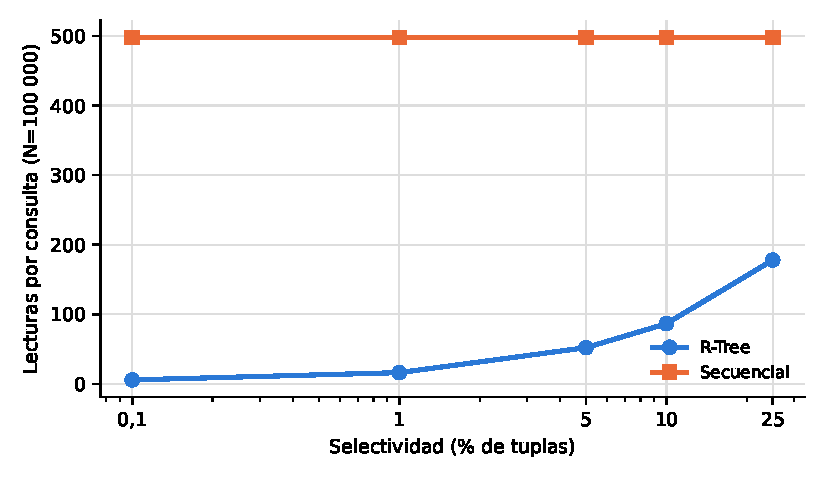
\includegraphics[width=0.75\textwidth]{exp5_radio.pdf}
  \caption{Lecturas por consulta para \code{WITHIN\_RADIUS} con \(N = 100\,000\).}
\end{figure}

\begin{center}
\begin{tabular}{rrrr}
\hline
 & \multicolumn{3}{c}{Lecturas por consulta} \\
\cline{2-4}
Selectividad & R-Tree (\(N=10^4\)) & R-Tree (\(N=10^5\)) & Secuencial (\(N=10^5\)) \\
\hline
0,1\,\% & 2,7 & 5,7 & 498 \\
1\,\%   & 4,5 & 16,3 & 498 \\
5\,\%   & 8,7 & 52,1 & 498 \\
10\,\%  & 13,6 & 86,6 & 498 \\
25\,\%  & 23,1 & 178,0 & 498 \\
\hline
\end{tabular}
\end{center}

\begin{itemize}
  \item El escaneo secuencial siempre lee las 498 páginas del Heap, sin importar
        la selectividad: su costo es \(P\).
  \item Con \(N = 100\,000\) y \(0{,}1\%\) de selectividad, el R-Tree lee 5,7
        páginas, unas 87 veces menos. Incluso con \(25\%\) de selectividad lee
        178, todavía por debajo del full scan.
  \item Al crecer \(N\), el R-Tree agrega niveles pero el costo crece mucho más
        despacio que \(P\): entre \(N=10^4\) y \(N=10^5\) las lecturas se
        duplican, mientras que el escaneo se multiplica por 10.
  \item La latencia sigue el mismo orden: para \(N=100\,000\) el R-Tree tarda
        entre 3 y 159 ms según la selectividad, frente a \(\approx 197\) ms del
        escaneo completo.
\end{itemize}

\subsubsection{k vecinos más cercanos}

\begin{figure}[htbp]
  \centering
  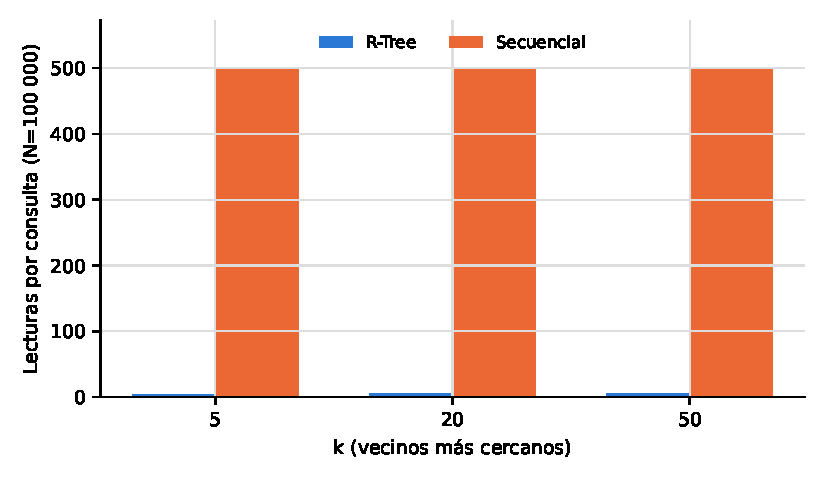
\includegraphics[width=0.75\textwidth]{exp5_knn.pdf}
  \caption{Lecturas por consulta para \code{KNN} con \(N = 100\,000\).}
\end{figure}

\begin{center}
\begin{tabular}{rrrr}
\hline
 & \multicolumn{3}{c}{Lecturas por consulta} \\
\cline{2-4}
\(k\) & R-Tree (\(N=10^4\)) & R-Tree (\(N=10^5\)) & Secuencial (\(N=10^5\)) \\
\hline
5  & 3,5 & 4,6 & 498 \\
20 & 4,0 & 5,0 & 498 \\
50 & 4,6 & 5,6 & 498 \\
\hline
\end{tabular}
\end{center}

El costo del R-Tree es casi constante: la cola de prioridad baja por una rama y
poda el resto en cuanto la cota inferior supera al \(k\)-ésimo vecino. Pasar de
\(k=5\) a \(k=50\) agrega apenas una página. El escaneo, en cambio, no puede
evitar leer la tabla completa y además ordena \(N\) distancias: con
\(N=100\,000\) tarda \(\approx 279\) ms por consulta, frente a \(\approx 1\) ms
del R-Tree. La diferencia en lecturas es de 498 a 4,6 páginas.

\subsubsection{Maldición de la dimensionalidad}

\begin{figure}[htbp]
  \centering
  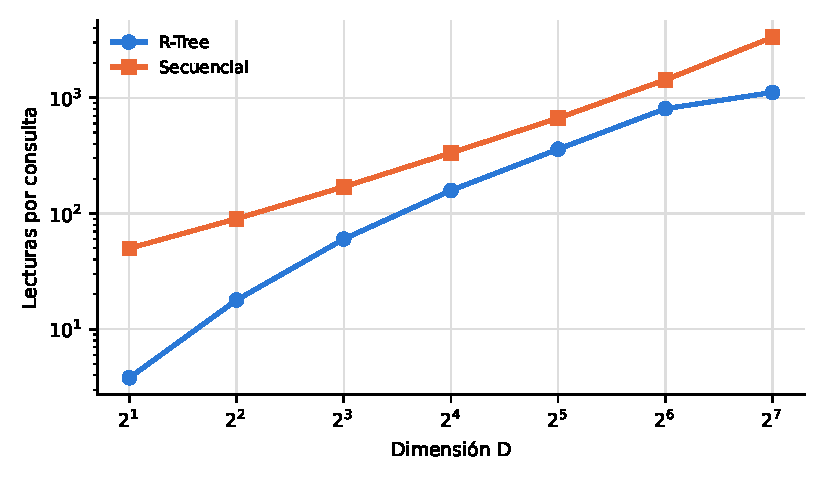
\includegraphics[width=0.75\textwidth]{exp5_dimension.pdf}
  \caption{Lecturas por consulta según la dimensión del R-Tree (\(N = 10\,000\)).}
\end{figure}

\begin{center}
\begin{tabular}{rrrr}
\hline
\(D\) & Lecturas R-Tree & Lecturas full scan & Filas devueltas \\
\hline
2   & 3,8    & 50    & 96,2 \\
4   & 17,9   & 90    & 76,5 \\
8   & 60,1   & 170   & 26,3 \\
16  & 158,3  & 334   & 4,0 \\
32  & 359,6  & 667   & 1,0 \\
64  & 804,6  & 1\,429 & 1,0 \\
128 & 1\,112,5 & 3\,334 & 1,0 \\
\hline
\end{tabular}
\end{center}

\begin{itemize}
  \item Hasta \(D=4\) el R-Tree lee entre 4 y 5 veces menos que el full scan.
  \item A partir de \(D=8\) los MBR se solapan casi por completo: la poda deja
        de ser selectiva y el árbol termina visitando una fracción grande de las
        hojas.
  \item Con \(D=128\) el R-Tree todavía lee menos que el escaneo, pero la ventaja
        se reduce a un factor de 3 y el árbol ocupa muchos más niveles. Es el
        comportamiento esperado: los índices multidimensionales dejan de ser
        útiles cuando la dimensión se acerca al número de filas por página.
\end{itemize}

\subsection{Conclusiones}

\begin{itemize}
  \item El R-Tree reduce el costo de \code{WITHIN\_RADIUS} de \(O(P)\) a
        \(O(\text{hojas visitadas})\), con una ventaja de hasta dos órdenes de
        magnitud en consultas selectivas.
  \item \code{KNN} mantiene un costo casi constante respecto de \(k\), porque la
        cota \code{MINDIST} poda las ramas que no pueden mejorar al vecino actual.
  \item La poda por MBR funciona bien en 2D y se degrada con la dimensión: el
        experimento reproduce la maldición de la dimensionalidad.
  \item Persistir el árbol en páginas de tamaño fijo y reutilizar el
        \code{Pager} mantiene el conteo de I/O exacto y permite comparar el
        índice con el escaneo secuencial en igualdad de condiciones.
  \item La reconstrucción tras \code{DELETE} y reorganización es el precio de
        usar RID físicos; a cambio, resolver una fila cuesta una sola lectura.
\end{itemize}

